\documentclass[11pt]{report}
\usepackage{fancyhdr}
\usepackage{fancybox}
\usepackage{tipa}
\usepackage{framed}
\usepackage[retainorgcmds]{IEEEtrantools}
\usepackage[utf8x]{inputenc}
\usepackage{epsfig}
\usepackage{anysize}
\usepackage{gensymb}
\usepackage{amssymb}
\usepackage{graphicx}
%\usepackage[demo]{graphicx}
\usepackage{caption}
\usepackage{subcaption}
\usepackage[utf8x]{inputenc}
\usepackage{longtable}
\usepackage{url}
\usepackage{plain}
%\renewcommand{\bibname}{References}
%\usepackage{hyperref}
\usepackage[plainpages=false]{hyperref}
\hypersetup{
    colorlinks=true,
    linkcolor=black,
    citecolor=black,
    filecolor=black,
    urlcolor=black,
}
\lhead{}


\setcounter{page}{-100}
\setcounter{secnumdepth}{5}

\newenvironment{fminipage}%
{\begin{Sbox}\begin{minipage}}%
{\end{minipage}\end{Sbox}\fbox{\TheSbox}}
% Title Page
\title{\textbf{Checking Misuse in DroidRacer Traces using RWFM Model}}
\vspace{2.5cm}
\author{\bf{A R\&D Report}\\
        \\
        \emph{Submitted in partial fulfillment of requirements for degree of}\\
        \\
        \bf{Masters of Technology}\\
        \\
        \emph{by}\\
        \\
		\bf{Asif Ali}\\
        \bf{Roll No : 143059009}\\
        \\
        \emph{under the guidance of}\\
        \\
        \bf{Prof. R.K. Shyamasundar}\\
        \\\\
        
\includegraphics[height=3.5cm]{./images/iitb_logo}\\
        \\
        \bf{Department of Computer Science and Engineering}\\
        \bf{Indian Institute of Technology, Bombay}\\
}
\date{May, 2016}


% page layout settings

% \setlength{\parindent}{2pc}
% \setlength{\oddsidemargin}{50pt}
% \setlength{\evensidemargin}{50pt}
% \setlength{\marginparwidth}{50pt}
% \setlength{\textheight}{9.0in}
% \setlength{\topmargin}{-0.75in}
% \setlength{\footskip}{30pt}

\marginsize{2.5cm}{2.5cm}{1cm}{1.5cm}
\setlength{\headheight}{15pt}

\pagestyle{fancy}

\usepackage{graphicx}
\begin{document}
\maketitle
\pagenumbering{roman}
\tableofcontents
%\listoffigures
%\listoftables
\begin{abstract}
 Smartphone are become integral part of our life.This is possible because the smart-phone operating system allows third party application to use system API for completing its job.
the major player in the smart-phone segment is ANDROID.which cover over 80 \% of total smart-phone market share and got millions of application in its play store .However it also has its Dark side.
There are thousands of malicious application in play store which can steal your credential and exploit the weakness of security policies in the ANDROID O.S.
So in order to solve this we are using RWFM model to assure the android security . 
\end{abstract}
\pagebreak

\chapter{Introduction}
Most of the android developers are using third party libraries in their applications. For example 50\% of the free apps embed third party libraries ( like advertisement libraries etc.). 
They may used by developers to provide various features at significant reduced time and cost. For example in app purchases, PDF view, cloud computing etc.
\par Many third party libraries access privacy-sensitive information even without notification to users or application developers. For example over the analysis of 1,00,000 android
apps reveals that third party libraries covertly utilize Andrid APIs to access privacy-sensitive resources such as GET\_ACCOUNTS, READ\_PHONE\_STATE or READ\_CALENDAR without mentioning
them properly in their Developer’s Guide. The current Android platform provides coarse-grained controls for regulating whether third party libraries access private information, allowing
them to operate with the same permission as their host apps.
\par In these days most of our daily work has been handled by applications. These applications handled different types of data. Thse data can be of differ sensitivity(belong to different
security levels). The security mechainism working today are insufficient to overcome differentiate between these sensitivity. RWFM (Reader Writer Flow Model) offers a simple, intutive
and systematic approach to track down the flow of information amongst the subjects in a system variety basis. We present an script which work on RWFM to track down readers and writers of information very explicitly.
Our script tracks down flow of information using explictly labelling each entiy in a communication( usually in form of subjects and objects). 

\chapter{Reader Writers Flow Model} 
In this section, we introduce RWFM model,which is  novel model  for information flow control. RWFM is ovtained by recasting the DEnning's label model. RWFM can be definded as five tuples
                          , where S and O denote the set of subjects and objects in the information system respectively.\
RWFM describes following operations under which operation is as follows:
\textbf{READ RULE}
Subject s with label (s1,R1,W1) requests read access to an object o with label (s2,R2,W2).
if(s R2) then 
\par change the label of s to (s1,R1 R2,W1 W2)
\par allowing
ELSE 
\par DENY

\textbf{WRITE RULE}
Subject s with label (s1,R1,W1) requests write access to an object o with label (s2,R2,W2).
If(s W2 R1 R2 W1 W2) then 
\par allowingELSE 
\
\subsection{Libraries abusing undocumented permissions}
\par App developers knows what third party library will use based on its permissions required in the documentation, specifying its must-have permissions and optionally required 
permissions. Due to lack in in-app privilege separation app can take permissions(as its host app) which were not mention in their documentation. If third party library dynamically
checks whether it has certain permission it can abuse those permission without notifying users.
\subsection{Contaminated libraries}
\par Sometimes the libraries are legitimate but adversary is able to rewrite its binary or source code and redistribute it. App developer who uses these contaminated library code 
to develop the app are more vulnerable to privacy leaks, and may suffer monetary damage.
\subsection{Vulnerable libraries}
\par A third party may execute a class or javascript code downloaded from internet at runtime. If the mobile is connected to unsafe network and file is not encrypted the malicious
code can be replaced by the attacker. Such a malicious code can exploit host app permissions to leak personal informations.
\section{Real World Findings}
\par We investigate different characteristics of several third party libraries berief summary of which is given below:
\begin{description}
 \item[$\bullet$] 17 of 20 popular apps uses undocumented permissions.
 \item[$\bullet$] 72\% of 295 third party libraries rely on dynamic code executions.
 \item[$\bullet$] 17\% of 295 third party libraries uses JNI(Java Native Interface).
\end{description}

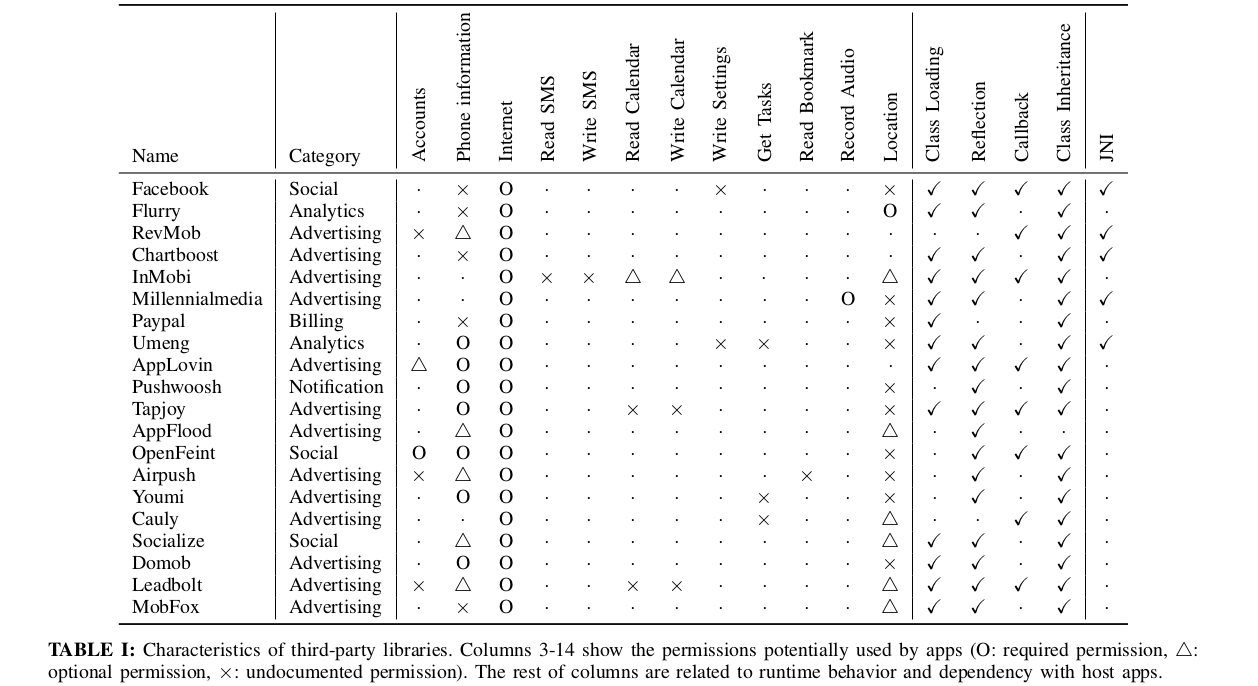
\includegraphics[width=150mm]{./images/table-1.png}
\par Table -1 summarizes the results of our findings for third party libraries used in 1,00,000 Android apps. 20 of the top popular which use at least one permissions out of 16 
permissions mentioned above.
\section{Thread Model}
\par FlexDroid assumes all third party libraries are malicious and their code and logic are not visible to developers and they might use dynamic features of java language.

\chapter{FlexDroid Design}
\section{Overview}
\par FlexDroid is a type of new permission system that adjusts the permissions of Android apps dynamically so as to enforce fine-grained controls of untrusted application modules.\par
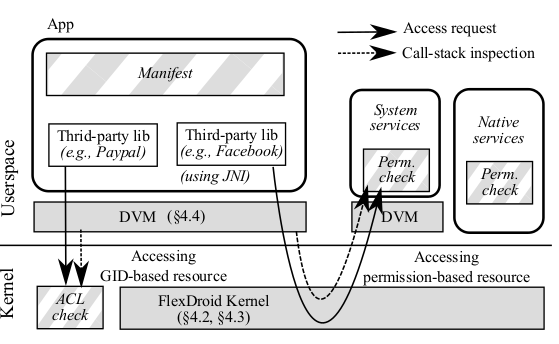
\includegraphics[width=90mm]{./images/fig-1.png}\newline
Key features of FlexDroid are as follows(as given in figure-1)
\begin{description}
 \item[$\bullet$] App developers specify a set of permissions for each individual module in android manifes file.
 \item[$\bullet$] Upon request of resource access,  FlexDroid identifies the context of execution by inspecting the Dalvik call stack.
 \item[$\bullet$] FlexDroid then determines whether to accept or decline the request according to permissions commonly granted to the modules.
\end{description}
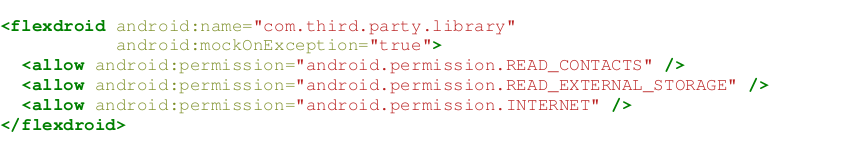
\includegraphics[width=150mm]{./images/fig-2.png}\newline
FlexDroid provide programming interface to developers in the form of simple XML manifes rules, to restrict third party library privileges. Figure 2 shows an 
example rule in FlexDroid’s policy. FlexDroid provides a \textbf{\it mockOnException}  attribute to enable developers to choose whether FlexDroid should offer mock data( ex. fake IMEI code) 
upon a request for an unauthorised resource.
\section{Challenges}
\par Achieving the above feature for a wide range of Android Apps presents several challenges:
\subsection{Secure Inter-Process Stack Inspection}
\par Android performs permission checking in a separate address space to protect memory tampering or in the kernel to secure the use of low level system calls and FlexDroid does so too.
FlexDroid require extra information to understand the context for fine-grained access control. To do that FlexDroid creates extra thread called \textbf{\it stack tracer},  that collects Dalvik 
call trace and send it to the permission checker upon request. It is also possible that malicious third-party library may also create the same name thread and send fake call data 
trace. To protect from that FlexDroid uses secure transmission channel between individual stack tracer thread and permission checker and ignores all attempts to use stack transmission
channel except those by the stack tracer.
\par The detailed procedure of the inter-process stack inspection differs according to the type of requested resource. Android resource broadly fall into two categories: user-space and kernel spcace depending upon which component they are responsible for access control.
\begin{description}
\item [User-space Resources:]
\par Apps access userspace resources through interfaces provided by the Android system services. Such resources include system resources(GPS,camera etc.) and app components 
(activity, service, content provider, and broadcast reciever).
\par In Android, when an app requests to access a resource to a corresponding system service ( eg. Location Manager), the system service process queries the PackageManager(PM) to 
see whether  the app has proper permission. FlexDroid provides inter-process stack inspection to conduct access control at the granularity of a module. Upon request from PM, the 
stack tracer of the app passes Dalvik call trace to PM via secure stack transmission channel mentioned above. PM then looks through all the modules involved in the current access 
request to find out the granted permission among them.
\item [Kernel-space Resources:]
\par Apps access kernel resources (Internal ,external strage,Bluetooth etc) via system calls. In Android, unlike the user-space resource case, PM does not conduct permission 
checking  for kernel level resources. Instead at the initialisation of an app, PM passes a set of permissions checking itslef, using Linux’s Access Control List(ACL). FlexDroid 
enforces the kernel to conduct inter-process inspection through the stack transmission channel during permission checking. Additionally , upon installation, PM sends to the kernel 
a set of granted permissions to each module in the app so as to avoid expensive user-kernel communications later on.
\end{description}
\subsection{Ensuring Dalvik Stack Integrity against Native Code}
\par Android supports the Java Native Interface and allows developers to parts of an app or library to incorporate native libraries.
\par Despite its advantages, it renders memory safety of Java programming language obselete, which results in security threats in Android. Some of the possible attacks by malicious
JNI code are as follows:
\begin{description}
 \item [Compromising the stack trace] \par An attacker can effectively guess the address of a memory region used by stack tracer and manipulate the content.
 \item [Manipulating Dalvik stack] \par An attacker can directly manipulate Dalvik stacks, thereby corrupting the integrity of the call stacks used for inspection.
\end{description}

\par \textbf{Defenses}
\begin{description}
 \item [Process Separation:]
	Process separation naturally supports sandboxing. Since it lets JNI thread run in a separate process, JNI code is not able to access the region of Java code is not able to
	access the memory region of java code directly.
 \item [Software fault Isolation(SFI):]
	SFI restricts memory accessible by JNI through masking the operands of store and jump instructions used in JNI.	
 \item [Hardware fault Isolation(HFI):]
	FlexDroid uses HFI approach to implement JNI sandboxing, as the process separation and SFI approaches significant overheads compared to HFI. We introduced two memory 
	domains, JNI and Java which represent restricted memory regions assigned for JNI and Java code respectively.	
\end{description}
\par But there are many challeges in applying this design of FlexDroid. In the default setting, when JNI attempts to access memory regions for the stack, heap, and shared  
libraries at the java domain, JNI domain fault occurs since only JNI can access JNI domain. To overcome this, FlexDroid provides the JNI domain with separate stack and heap and 
loads a set of necessary shared libraries at the JNI domain.
\par Similary FlexDroid divides the pointer variables as valid or potentially malicious pointers and disallows latter ones to be passed to java code via Java API. 
FlexDroid manages a table called Valid Address Table (VAT) that maintains a list of memory addresses which have been returned from Java code via Java API calls.
\subsection{Dynamic Permission Management}
\par Java Reflection is a feature in Java which allows programmers to inspect or modify any code at run time across Java classes for various benefits. At the same time it creates 
a lot of problem for creating the mapping between modules and permissions accurately. For example, a third party library may create and run the code dynamically using reflection as
host module.
\par
\chapter{Experimental Setup}
\subsection{System Configurations}
\begin{description}
 \item[$\bullet$]Nexus 5 (2.265 Ghz quad core CPU 2GB RAM)  
 \item[$\bullet$]FlexDroid
 \item[$\bullet$]Android 4.4.4(KitKat)
\end{description}
\subsection{Experiment}
\par We searched out 32 top apps from App Annie and downloaded it, from Google Play store.
Then we ran out these apps in Android with and without FlexDroid, and checked to see if an app crashes during the execution.

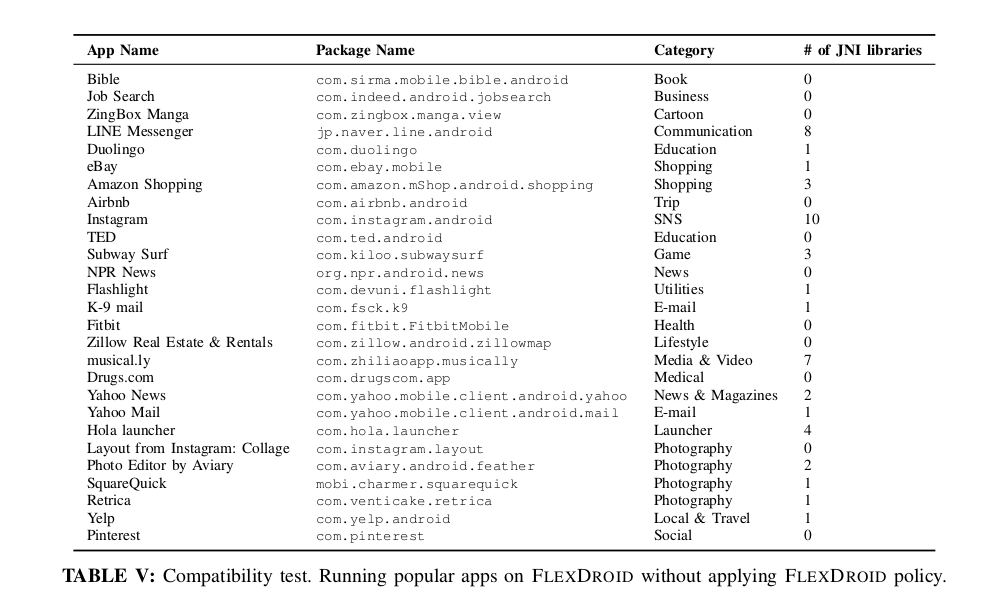
\includegraphics[width=120mm]{./images/table-5.png}\newline

\par Table-5 shows a list of apps run as normal in presence of FlexDroid. But some apps are there which doesn’t run with FlexDroid app. Those apps were 
Waze Social GPS Map and Travel(com.waze), Uber(com.ubercab),Adobe Acrobat Reader(com.adobe.reader), Facebook(com.facebook.katana), UC Browser(com.UCMobile.intl).The problem we 
searched out was coming from JNI sandbox.Then we found that root of the fault was PthreadID,mmap() and free(). JNI code of Waze fails because in the safety check, it compares the 
Pthread ID obtained from Java to the thread id coming from JNI code. Since both are not the same it came to crash. Separating Pthread Id from thead structure was a way to avoid 
this problem, although it requires modification of JNI code.
\par Uber employs a JNI library SnappyDB which is a key-value database for Android. It maps data stored in a file to memory pages using mmap(). 
Since memory pages are out of JNI domain, it generates domain faults.
Allocating memory to each separate region depending upon the caller of mmap() is our future work.
\par When executing JNI code of Adobe Acrobat Reader, free() was creating problem. We haven’t figure what creating this fault but we beleive that we will solve it through 
engineering.



\begin{thebibliography}{100} % 100 is a random guess of the total number of
%references
\addtolength{\leftmargin}{0.2in} % sets up alignment with the following line.
\setlength{\itemindent}{-0.2in}
\bibitem{permission} K. W. Y. Au, Y. F. Zhou, Z. Huang, and D. Lie. Pscout: Analyzing the android permission specification. In Proceedings of the 2012 ACM Conference on Computer and Communications Security, 2012.
\bibitem{berestford} A. R. Beresford, A. Rice, N. Skehin, and R. Sohan. Mockdroid: Trading privacy for application functionality on smartphones. In Proceedings of the 12th Workshop on Mobile Computing Systems and Applications,2011.
\bibitem{boraskar} R. Bhoraskar, S. Han, J. Jeon, T. Azim, S. Chen, J. Jung, S. Nath,R. Wang, and D. Wetherall. Brahmastra: Driving apps to test the security of third-party components. In 23rd USENIX Security Symposium, Aug.2014.
\bibitem{acl} acl Linux man page. \url{http://linux.die.net/man/5/acl.}
\bibitem{actionbaserlock} Actionbarsherlock Android SDK.\url{ http://actionbarsherlock.com/.}
\bibitem{pdflibrary} Adobe Pdf Library SDK. \url{http://www.adobe.com/devnet/pdf/library.html.}
\bibitem{apk-tool} android-apktool: A tool for reverse engineering Android apk files. \url{https://code.google.com/p/android-apktool/.}


\end{thebibliography}

\end{document}